%!TEX root = series of tubes.tex
\begin{figure*}
\centering
    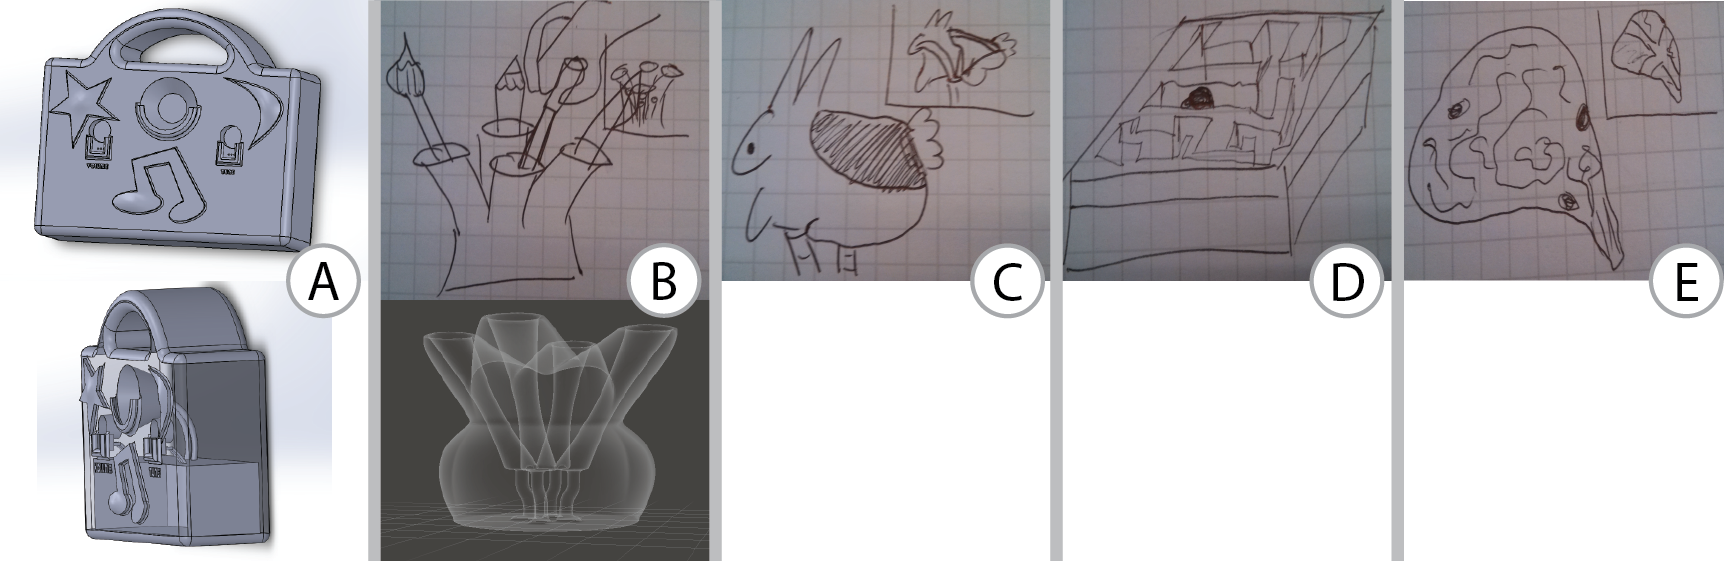
\includegraphics[width=7in]{figures/examples.png}
\caption{A series of example objects created using our system.  (a) is a touch-sensitive brain toy.  (b) is a rabbit which ``breathes'' using wind pipes we built.  (c) shows a portable radio.  (d) shows a presence-aware pen holder.  (e) is a maze game.}
\label{fig:examples}
\end{figure*}

\section{Totally Tubular Example Objects}
To evaluate and highlight our tool's capabilities, we fabricated a set of six prototype objects designed using \systemnamenospace.  To show that our approach is printer-independent, we fabricated some on a Makerbot Replicator 2 and the rest on an Objet Connex 260.  Each prototype object explores the expansion of an existing sensing or actuation technique to the surface of 3D printed objects.
%All prototypes were fabricated in a single piece, unless described otherwise. \bjoern{2 of 5 will have been fabricated otherwise -  Radio, Neon sign - both in pieces.}

\subsection{Touch-sensitive Toys (open, liquid, star, endpoint)}

To expand Touch\'{e} \cite{Sato-touche} to 3D printed forms, we created a set of touch-sensitive toys and a companion app that identifies the objects as well as touched parts of the objects (inspired by \cite{Harrison-acoustic}). The objects --- a brain and boat, in our example --- can be set on a base, upon which the computer displays ``brain'' or ``boat''. Touching the brain model's front protrusion yields the announcement ``olfactory bulb''. The distinct touch points on each object are connected by an interior star topology, and touch sensing is performed via a single conductive connection to the base, using swept-frequency capacitive sensing (see Figure \ref{fig:examples}a). %We built a smart base which can distinguish between the toys and also determine which toy is mounted:
Since each toy and each gesture has a distinct capacitive signature, we use a simple classifier trained to detect both toy and gesture based on profile.

The models we used for the toys were downloaded from the  Thingiverse website. \bjoern{I thought the brain model came from Berkeley?} We then used \systemname to create the desired internal pipes. All components were fabricated on a Makerbot, support-free.  After printing, we injected copper paint (CuPro-Cote) into the interior pipes using a craft syringe.  This paint requires approximately 2 days to fully dry in this configuration (3mm diameter tubes, maximum tube length 10cm).  Our smart base is powered by an Arduino Uno running open-source SFCS code\footnote{\url{http://www.instructables.com/id/Touche-for-Arduino-Advanced-touch-sensing}}. \bjoern{If we don't have appendices, insert resistance measurement for this paint here.}

\subsection{Breathing Bunny (semi-closed, gas, endpoint)}

With inspiration from PneUIs \cite{Yao-pneui} for using gases to both provide sensation to the user through openings and deform a model internally, we created a rabbit with a pair of tubes that can simulate breathing (see Figure \ref{fig:examples}b).  When the rabbit inhales through its nose, its abdomen rises, and as it exhales its abdomen falls.  For this, we used a combination air/vacuum pump (ROB-10398): one terminal creates a vacuum while the other creates positive pressure.  
The rabbit model, the well-known Stanford Bunny\footnote{\url{http://en.wikipedia.org/wiki/Stanford_bunny}}, was downloaded from Thingiverse. We then used \systemname to add two pipes: one open pipe exiting at its mouth, and one semi-closed pipe capped at its abdomen.  We connected one pipe to each of our pump's terminals, and using a programmable power supply we mimic a rabbit's breathing pattern.  This example was printed on the Objet using a flexible material and its support material was flushed post-print.

\subsection{Custom Radio (open, threadable, endpoint)}
A custom radio (Figure \ref{fig:examples}c) shows how pipes can be used to integrate electronic components into the user-facing surface of an object. The radio includes a power and volume dial, and LED which goes on when the radio is on, and a tuner dial. An Arduino Pro Micro microcontroller, Si4703 FM tuner, and 6V (4xAA) power supply are embedded in the base of the radio. The sound is played through a single .5 Watt speaker.

The radio shell was modelled in SolidWorks. We included slots on the 3D model matching the shape of the electronic components that were to be embedded. The model was then imported into \systemnamenospace, where we created a network of 8 individual open pipes (3 per potentiometer, 1 for the LED, 1 for the speaker) to connect the components to the base of the radio. We fabricated the radio itself on our Makerbot, support-free, but cut in two pieces to allow the Arduino and battery pack to be inserted. We then threaded the pipes with wires to connect the components to the microcontroller at the base of the radio. 

\subsection{Presence-aware Pen Holder (open, threadable, endpoint)}
Our presence-aware pen holder can distinguish which tool or tools a user has picked up (see Figure \ref{fig:examples}d).  Our pen holder uses a modification of the FlyEye technique described by Wimmer \cite{Wimmer-flyeye} in which an IR camera senses a user's grasp on an object, getting data from IR light transmitted on fiber optic cables.  We marry this technique here with the Sauron technique \cite{Savage-sauron}: instead of using mirrors to redirect light and motion sensing as Sauron does, we use fiber optic cables. \bjoern{I think people remember Sauron as being all about hollow objects and we use ray-tracing to know how reflected light will travel; using fiberoptics seems not that closely related, other than its use of optical sensors.}

The penholder body was created in Solidworks. We used \systemname to add four internal open pipes connecting each pen chamber to the based on the pen holder. This prototype was built on our Makerbot support-free.  Each pipe was then threaded with a fiber optic cable.  We use a single cable per pipe; our 6mm diameter fiber optic cables, in comparison to the fine tubes used in the original work, can emit and receive through the same cable because their cross-sectional area is large enough to accommodate both functions \bjoern{still unclear how this actually works; I'm a little worried about having any vague statements about fiber optics as Patrick could get this paper}. At the base of each tube is a QRE1113 line sensor digital breakout board, which has an integrated IR emitter and receiver.   When a pen is in its appointed place, the emitted infrared light is reflected off its bottom and travels back to the receiver, where it registers as bright.  

\subsection{Maze (fully enclosed, particulate, tree, path)}

We created a maze game with a marble that can be navigated through a maze-like path, with exits on either side of the model (Figure \ref{fig:examples}e). 

The maze is based on an SVG file we manually created and processed with our internal path routing tool.  We printed the maze on the Objet using a transparent material \bjoern{bottom doesn't look transparent}. The final artifact was fabricated in two halves fastened together via glue, to allow removal of support material with a high-pressure water tool.  We plugged the ends of the tubes post-print with additional material to ensure the ball does not escape.

\subsection{Animated Neon Sign (open, threadable, fully constrained)}

\begin{figure}[t]
\centering
    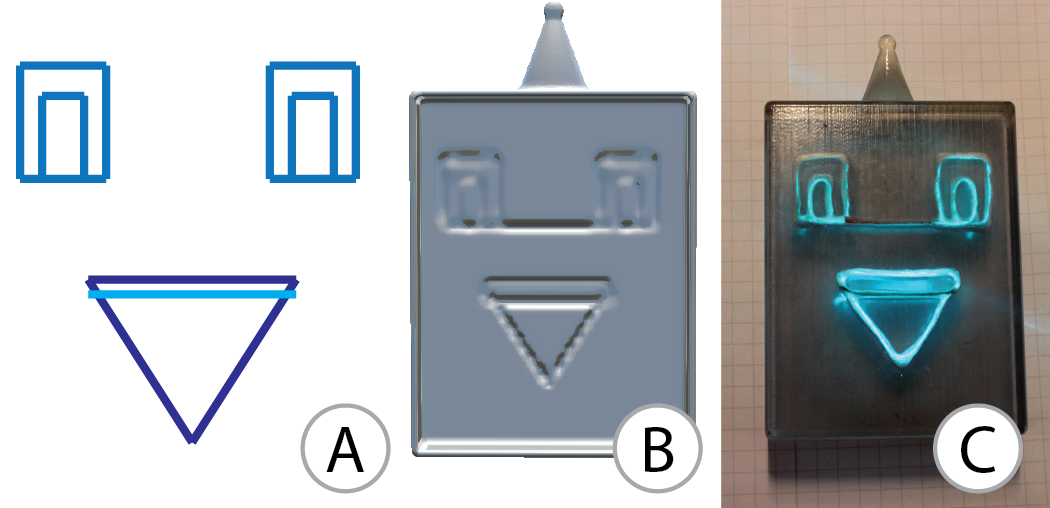
\includegraphics[width=3.4in]{figures/sign.png}
\caption{A two-state animated neon sign designed using our tool.  (a) shows the input SVG files, with the eyes (non-animated) in black and the two states of the mouth in {\color{blue}blue} and {\color{gray}gray}.  (b) shows the resultant mesh when we subtracted the generated tubes, with rear exit tubes circled in {\color{blue}blue} \valkyrie{fix this with boolean magic}. In (c), we show the fabricated sign.}
\label{fig:neon}
\end{figure}

Neon art is traditionally made from hand-formed glass tubes containing neon gas.  The tubes light up when a current is passed through them.  For this type of art, the path of the tubes is of crucial importance, as it determines how the sign will look.  We designed a custom neon robot head which can be animated to ``talk''. 
The external geometry of the model was imported into \systemnamenospace, which created the associated pipes using its internal path routing tool.  We added additional endpoint-constrained tubes as exits out the rear of the model to allow us to hide the controls (see Figure \ref{fig:neon}B).  We then printed the model on the Objet using transparent material. The model was printed in two halves, cutting through the plane of the internal path, to facilitate assembly. 

The pipes are threaded with electroluminescent wire which is lit in sequence, using an EL wire sequencer, to create the animation.